\chapter{Modelling} \label{sec:modelling}


\section{Interior Magnet PMSM \label{sec:model_pmsm}}

Starting point of this derivation is the stator voltage equation in the stationary reference frame (SRF). The stator voltage space vector $\underline{u}_S^S = u_{\alpha}+\J u_{\beta}$ is given by Faraday's law of induction with the magnetic stator flux linkage ${\underline{\psi}}_S^S $ and the stator current space vector $\underline{i}_S^S = i_{\alpha}+\J i_{\beta}$.
\begin{equation}
	\underline{u}_S^S = R_S \underline{i}_S^S + \dot{\underline{\psi}}_S^S 
	\label{equ:1_voltage_equation_SRF}
\end{equation}
Assuming the stator resistance $R_S$ has rotational symmetry, Equation \eqref{equ:1_voltage_equation_SRF} is transferred to the rotor-fixed reference frame (RRF) using  $\underline{z}^{S}=\underline{z}^{R}e^{\J\varphi}$ .

\[
%\underbrace{
\underline{u}_S^R e^{\J \varphi}
%}_{\underline{u}_S^R}
=
R_S
%\underbrace{
\underline{i}_S^R e^{\J \varphi}
%}_{\underline{i}_S^R}
+
\frac{\diff}{\diff t}
\left(
\underline{\psi}_S^R e^{\J \varphi}
\right)
\]
For the contribution of the flux linkage space vector, the chain rule  for the differentiation has to be applied.

\begin{equation}
    \begin{split}
        \frac{\diff}{\diff t}
        \left(
        \underline{\psi}_S^R e^{\J \varphi}
        \right)
        &=
        \dot{\underline{\psi}}_S^R e^{\J \varphi}
        +
        \J \dot{\varphi}
        \underline{\psi}_S^R e^{\J \varphi} \\
        &=
        \left(
        \dot{\underline{\psi}}_S^R
        +
        \J \omega\underline{\psi}_S^R
        \right)e^{\J \varphi}
    \end{split}
    \label{equ:1_diff_psi}
\end{equation}
With $\omega = \dot{\varphi}$ being the electrical rotor speed.  The additional speed-dependent term $\J\omega\underline{\psi}_S^R$ represents the voltage induced by expressing the flux linkage in the rotating reference frame. \\
\[
\underline{u}_S^R e^{\J \varphi}
=
\left(
R_S
\underline{i}_S^R
+
\dot{\underline{\psi}}_S^R
+
\J \omega\underline{\psi}_S^R
\right)e^{\J \varphi}
\]
Next, the voltage equation for the rotating reference frame can be written as

\begin{equation}
	\underline{u}_S^R = R_S \underline{i}_S^R + \underline{\dot{\psi}}_S^R + \J  \omega \underline{\psi}_S^R
	\label{equ:1_voltage_equation_RRF}
\end{equation}
In the \acrshort{rrf}, the flux linkage of the permanent magnet $\psi_{PM}$ is aligned with
the $d$-axis. The stator flux linkage is given by the superposition of the space vectors of flux linkage due to the permanent magnets and Ampere's law for the stator current. To stay within the framework of complex space vectors no saliency $L_d = L_q = L_S$ is considered for now\footnote{Otherwise the real-valued vector analog of Equation \eqref{equ:1_superpos_Li_psi}, $\bm{\psi}_S^R = \bm{L}_S \bm{i}_S^R + \bm{\psi}_{PM}^R$ with $\bm{L}_S \in \mathbb{R}^{2\times2}$, would have to be used to adequately capture the effects of different $d$- and $q$-axis inductance.}. 

\begin{equation}
    \begin{split}
        \underline{\psi}_S^R
        &=
        L_S\underline{i}_S^R
        +
        \underline{\psi}_{PM}\\
        &=
        L_S\underline{i}_S^R
        +
        \left(
        \psi_{PM}+\J 0
        \right)
    \end{split}
    \label{equ:1_superpos_Li_psi}
\end{equation}
Under the assumption that the permanent magnet flux linkage change due to temperature over time is negligible, $\psi_{PM}$ is constant. Therefore, inserting Equation \eqref{equ:1_superpos_Li_psi} into \eqref{equ:1_diff_psi} leads to

\[
\frac{\diff}{\diff t}
\left(
\underline{\psi}_S^S e^{\J \varphi}
\right)
=
L_S\dot{\underline{i}}_S^R
+
\left(
\J \omega L_S\underline{i}_S^R
+
\J \omega\psi_{PM}
\right).
\]
Substituting this result back into the Stator Voltage Equation \eqref{equ:1_voltage_equation_RRF},

\[
\underline{u}_S^R
=
R_S\underline{i}_S^R
+
L_S\dot{\underline{i}}_S^R
+
\J \omega L_S\underline{i}_S^R
+
\J \omega\psi_{PM}.
\]
Collecting terms and writing the space vectors explicitly,

\[
u_{Sd}+\J u_{Sq}
=
\left(
R_S+\J \omega L_S
\right)
\left(
i_{Sd}+\J i_{Sq}
\right)
+
L_S
\left(
\dot{i}_{Sd}+\J \dot{i}_{Sq}
\right)
+
\J \omega\psi_{PM}.
\]
The stator inductance $L_S$ is commonly modeled as independent $L_d$- and $L_q$-axes inductances. This is done  to properly capture the salient pole effects. Considering this, the voltage equation can be split into its $d$ and $q$ components:

\begin{equation}
    \begin{split}
        u_{Sd}
        &=
        R_S i_{Sd}
        +
        L_d\dot{i}_{Sd}
        -
        \omega L_q i_{Sq}\\
        u_{Sq}
        &=
        R_S i_{Sq}
        +
        L_q\dot{i}_{Sq}
        +
        \omega L_d i_{Sd}
        +
        \omega\psi_{PM}
    \end{split}
    \label{equ:1_v_SRF_componentwise}
\end{equation}
Within the scope of this thesis $L_d, L_q$ and $\psi_{PM}$ is assumed to constant.


\subsection{State Space Model} \label{sec:1_pmsm_ss}
To solve for the current derivatives, the component-wise Voltage Equation in the \acrshort{rrf} \eqref{equ:1_v_SRF_componentwise} is rearranged:
\[
\dot{i}_{Sd} = \frac{1}{L_d}u_{Sd} - \frac{R_S}{L_d} i_{Sd} + \frac{L_q}{L_d}\omega_e i_{Sq}
\]
\[ 
\dot{i}_{Sq} = \frac{1}{L_q}u_{Sq} - \frac{R_S}{L_q} i_{Sq} - \frac{L_d}{L_q}\omega_e i_{Sd} - \frac{\psi_{PM}}{L_q}\omega_e \]
In matrix form, this yields the continuous time state-space model \eqref{equ:1_apv_ss}.
\begin{equation}
	\dfrac{\diff}{\diff t} \begin{bmatrix}
		i_{Sd} \\i_{Sq}
	\end{bmatrix}
	= \begin{bmatrix}
		-\frac{R_S}{L_d} & \frac{L_q}{L_d} \omega_e(t)\\ -\frac{L_d}{L_q} \omega_e(t) & -\frac{R_S}{L_q}
	\end{bmatrix}\begin{bmatrix}
		i_{Sd} \\i_{Sq}
	\end{bmatrix} + 
	\begin{bmatrix}
		\frac{1}{L_d} & 0 \\ 0 & \frac{1}{L_q}
	\end{bmatrix}\begin{bmatrix}
		u_{Sd} \\u_{Sq}
	\end{bmatrix} + \begin{bmatrix}
		0 \\ - \frac{\psi_{PM}}{L_q} \omega_e(t)
	\end{bmatrix}
	\label{equ:1_apv_ss}
\end{equation}
Defining the stator current vector as the state vector, $\begin{bmatrix}
		i_{Sd}  & i_{Sq}
	\end{bmatrix}^\T 
    = \bm{i}_S = {\bm x} $ 
and using established TUG notation for control system and highlighting the parameter-dependency in $\omega(t)$, this continuous time dynamical system is written as

\[
\dfrac{\diff}{\diff t} \begin{bmatrix}
		i_{Sd} \\i_{Sq}
	\end{bmatrix} 
    = \dot{\bm{i}}_S = \dot{\bm x} 
    = \bm{A}_c (\omega(t)) \x + \bm{B}_c \bm{u} + \bm{E}_c (\omega(t))
\]
Note that, the control signal $u$ will always refer to the stator voltage within the scope of this work.\\
Since a variety of state space systems are used in this thesis, the short notation 
\[
\Sigma_c : \left(\bm{A}_c \left(\omega \left(t\right) \right),\; \bm{B}_c,\; \bm{E}_c \left(\omega \left(t\right) \right) \right) 
\]
will also be used to refer to the same affine, parameter-varying continuous-time system.\\

\begin{comment}
    To analyze the Model \eqref{equ:1_apv_ss} in the context of linear parameter-varying systems, the permanent magnet flux linkage $\psi_{PM}$ is sometimes treated as a state or input \cite{plsAddRef}. This results in the following description, which matches the generic LPV system form as defined in \cite{lpvBriat} $\Dot{\x} = \bm{A}(\omega) \x  + \bm{B} (\omega)$.
\begin{equation}
	\dfrac{\diff }{\diff t} \begin{bmatrix}
		i_{Sd} \\i_{Sq}
	\end{bmatrix}
	= \begin{bmatrix}
		-\frac{R_S}{L_d} & \frac{L_q}{L_d} \omega_e(t)\\ -\frac{L_d}{L_q} \omega_e(t) & -\frac{R_S}{L_q}
	\end{bmatrix}\begin{bmatrix}
		i_{Sd} \\i_{Sq}
	\end{bmatrix} + 
	\begin{bmatrix}
		\frac{1}{L_d} & 0 & 0 \\ 0 & \frac{1}{L_q} & -\frac{\omega_e(t)}{L_q}
	\end{bmatrix}\begin{bmatrix}
		u_{Sd} \\u_{Sq} \\ \psi_{PM}
	\end{bmatrix}
	\label{equ:apv_ss_psi}
\end{equation}d
\end{comment}

Analyzing this model, one has to quantify the influence of the parameter $\omega$. Due to the balance of angular momentum of the motor shaft \eqref{equ:1_coupling}, the electrical rotor speed $\omega = \omega_e = \omega_{m1}p$ is Lipschitz-continuous. With the eigenvalues of the respective dynamical system \eqref{equ:1_coupling} being slower than \eqref{equ:2_apv_ss}, as discussed in Section \ref{sec:1_coupled_dyn}.


\section{Mechanical System \label{sec:model_coupling}}

The experimental evaluation of the model predictive current controller presented in this thesis will be conducted on an end-to-end testbed at TUG. As it will be explained in Section \ref{sec:ss_choice}, the dynamical system for the coupling will not directly be considered in the prediction of the MPC. Nevertheless,  the  electrical rotor speed of the  PMSM, which is linked with the amount of pole pairs $p$ to the mechanical speed, $\omega_{e} = p\omega_{m1}$ will influence its current dynamics, by means of a varying parameter or input, depending on the modeling. Consequently, the dynamics of the system of two coupled motors have to be analyzed, to adequately choose a prediction framework for the MPC.
\begin{figure}[H]
	\centering
	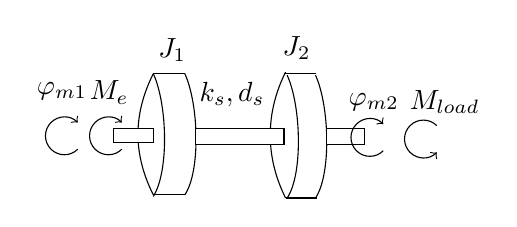
\begin{tikzpicture}[scale=2]


  \draw (1.14,-0.39) .. controls (1.01,-0.13) and (1.01,0.15) .. (1.14,0.41);


  \draw (0.5,-0.37) .. controls (0.6,-0.22) and (0.59,0.2) .. (0.5,0.4);

  \draw (0.3,-0.38) .. controls (0.4,-0.22) and (0.39,0.2) .. (0.3,0.4);

  \draw (1.33,-0.39) .. controls (1.43,-0.24) and (1.42,0.19) .. (1.33,0.39);

  \draw (1.15,-0.39) .. controls (1.25,-0.24) and (1.24,0.19) .. (1.15,0.39);

  \draw (0.3,-0.37) .. controls (0.17,-0.11) and (0.17,0.14) .. (0.3,0.4);

  \draw (0.3,0.40) -- (0.5,0.4);
  \draw (0.3,-0.37) -- (0.5,-0.37);
  \draw[fill=white] (0.05,-0.04) rectangle (0.3,0.05);

  \draw (0.57,-0.05) rectangle (1.13,0.05);

  \draw (1.13,0.4) -- (1.33,0.4);
  \draw (1.14,-0.39) -- (1.34,-0.39);
  \draw[fill=white] (0.57,-0.05) rectangle (1.13,0.05);
  \draw[fill=white] (1.4,-0.05) rectangle (1.64,0.05);


  \draw[->] (0.1,-0.08) arc[start angle=315, end angle=45, radius=0.12];
  \node at (0.02,0.28) {$M_e$};

  \draw[<-] (2.1,-0.1) arc[start angle=315, end angle=45, radius=0.12];
  \node at (2.15,0.22) {$M_{load}$};


  \draw[->] (-0.18,-0.08) arc[start angle=315, end angle=45, radius=0.12];

  \node at (-0.28,0.29) {$\varphi_{m1}$};


  \node at (1.7,0.22) {$\varphi_{m2}$};

  \node at (0.8,0.27) {$k_s,d_s$};

  \draw[->] (1.76,-0.09) arc[start angle=315, end angle=45, radius=0.12];

  \node at (0.42,0.55) {$J_1$};

  \node at (1.21,0.56) {$J_2$};


\end{tikzpicture}
	\caption{Diagram of a two mass oscillator.}
	\label{fig:0_mechS}
\end{figure}

The mechanical system, drawn in Figure \ref{fig:0_mechS}, is modeled as a two mass damped oscillator with $J_1$ as the moment of inertia of the PMSM and the $J_2$ for the load. Let $M_e$ be the electric torque, which is determined by 
\begin{equation}
    M_e = \frac{3}{2} p \left(\psi_{PM} i_{Sq} + \left(L_d - L_q\right) i_{Sq}i_{Sd} \right).
    \label{equ:1_pmsm_torque}
\end{equation}
Due to the elastic deformation of the shaft, the rotor position of both motors, $\varphi_{m1}, \varphi_{m2}$, can differ. The elastic coupling is modeled as a linear damped oscillator with $d_s$ being the damping coefficient and $k_s$ for the torsional stiffness of the shaft.  The values of the mechanical system used in the simulations can be obtained from Table \ref{tab:params_mechS}.\\

Isolating the left hand side of the Body Diagram \ref{fig:0_mechS} and applying the balance of momentum, with the oscillator acting on the differential speed $\Delta\omega_m = \omega_{m1} - \omega_{m2}$ and position $ \Delta \varphi_m = \int \Delta\omega_m \diff t$, leads to
\[
J_1 \frac{\diff(\omega_{m1})}{\diff t} = M_e - k_s \cdot \Delta\varphi_m - d_s \cdot \Delta\omega_m
\]
 The same is done for the right hand side, where the load torque $M_{load}$ acts:
 \[
 J_2 \frac{\diff(\omega_{m2})}{\diff t} = M_{load} + k_s\cdot \Delta\varphi_m + d_s \cdot  \Delta\omega_m
 \]
The dynamics of the mechanical system can then be written down as the following
\begin{equation}
	\begin{split}
			J_1 \frac{\diff(\omega_{m1})}{\diff t} &= M_e - k_s \cdot \Delta\varphi_m - d_s \cdot \Delta\omega_m \\
			J_2 \frac{\diff(\omega_{m2})}{\diff t} &= M_{load} + k_s\cdot \Delta\varphi_m + d_s \cdot  \Delta\omega_m \\
			\frac{\diff(\varphi_{m1})}{\diff t} &= \omega_{m1} \\
			\frac{\diff(\varphi_{m2})}{\diff t} &= \omega_{m2}
	\end{split}
	\label{equ:1_coupling}
\end{equation}

\section{Coupled System Dynamics} \label{sec:1_coupled_dyn}

To obtain one dynamical system of the PMSM interacting with the mechanical system, the Torque Relation \eqref{equ:1_pmsm_torque} is used to determine the electric torque, which acts as an input to the mechanical system. Using the balance of angular momentum and the load torque, the rotor speed can be determined, which in turn acts as an input on the PMSM via $\omega_e = \omega_{m1}p$.\\
Assuming a non-salient machine, $L_d = L_q = L_S$, the electrical time constant is given by $\tau_e = L_S/R_S$, which can be interpreted as a measure of how fast the stator current can change. For the mechanical system, a similar measure is the undamped natural frequency, which for a one-mass oscillator is given by
\[
\omega_{0,m} = \sqrt{\frac{k_s}{J}}.
\]
For the two-mass system of Equation \eqref{equ:1_coupling}, the reduced moment of inertia $J_{red} = J_1J_2/(J_1+J_2)$ is used, yielding the mechanical time constant
\[
\tau_{m} = \sqrt{\frac{J_{red}}{k_s}} = \omega_{m}^{-1}
\]
Using application-typical parameters, $\tau_e$ is smaller then $\tau_m$. This separation of timescales between the electrical and mechanical dynamics allows for the modeling assumptions in Section \ref{sec:ss_choice} regarding the consideration of $\omega$ as a slowly varying parameter in the prediction model. It should be noted that in some systems, $\tau_m$ may be close to $\tau_e$. The assumption that $\omega_e$ is constant may lead to prediction errors in these cases. Section \ref{sec:2_impl_sim} presents a simulation example in which the MPC cannot find a feasible solution under extreme conditions. In this case, the controller compensates for the unmodeled mechanical oscillations caused by changes in torque, while the voltage constraints remain active at all times.\\
The system parameters used in the simulations are listed in Table \ref{tab:params_mechS} and \ref{tab:params_NW3}.


